\begin{apendicesenv}

\partapendices

%
% Referencial Tecnológico da Prova de Conceito
%

\chapter[Referencial Tecnológico da PoC]{Referencial Tecnológico da PoC}
\label{apendice:referencial_tecnologico_poc}

O presente capítulo lista as tecnologias escolhidas ou envolvidas na criação da ferramenta.
da ferramenta Enpyre. Para as ferramentas de escolha, são apresentadas suas definições, suas vantagens e
suas limitações. Para as tecnologias associadas ao projeto por consequência, são apresentadas suas
definições.

\section{WebAssembly}

\subsection{Definição}

\href{https://webassembly.org/}{WebAssembly} é um bytecode portátil de baixo nível para Web. É desenvolvido de modo a ser independente de hardware e plataforma. Com o WebAssembly, existe a possibilidade de se compilar código de diversas linguagens em código de baixo nível. Atualmente existe suporte para C, C++, Rust entre outros.

O WebAssembly foi proposto de forma colaborativa por engenheiros de quatro grandes distribuidores de navegadores: Google, Microsoft, Mozilla e Apple. A implementação atual já é capaz de compilar uma quantidade grande de programas, mas existem ainda várias propostas em estudo para estender as funcionalidades da linguagem e a integração com JavaScript.

\subsection{Vantagens}

O WebAssembly é seguro, rápido, independente de hardware e plataforma, além de ser portátil e compacto. Em comparação, outras tecnologias que tentam ou tentaram a execução de código nativo na Web, como o ActiveX da Microsoft, o Native Client da Google, o Java da Oracle e o Flash da Adobe, falham ao alcançar pelo menos uma destas características.

\subsection{Limitações}

Dentre as limitações presentes no WebAssembly, está sua incapacidade de acessar diretamente o DOM, então qualquer manipulação de DOM deve ser feita com JavaScript. Além disso, o WebAssembly funciona apenas com uma única thread, e não tem acesso a todas as funções do navegador.


\section{Pyodide}

\subsection{Definição}

O \href{https://pyodide.org/}{Pyodide} é uma ferramenta que contém o interpretador do Python, em sua versão 3.9, sendo compilado para WebAssembly. Como resultado, é possível executar Python na Web, à partir de um navegador.

A ferramenta foi criada em 2018 por Michael Droettboom, desenvolvedor da Mozilla, inicialmente como parte do projeto Iodide. Este projeto propunha um ambiente de desenvolvimento baseado em navegadores, voltado para computação e programação científica e execução de notebooks do Jupyter. O projeto Iodide foi encerrado em Setembro de 2020, ainda podendo ser encontrado, mas não mais sendo mantido.

\subsection{Vantagens}

O Pyodide permite troca de informações entre os contextos JavaScript e Python. Por exemplo, é possível, usando JavaScript, manipular o DOM com informações obtidas do contexto do Python.

Para que a troca de informações entre contextos funcione, o Pyodide possui integrada uma conversão de tipos, que atua automaticamente durante o acesso de contexto do JavaScript para o Python ou vice-versa.

Além disso, é possível instalar dependências usando uma abstração do gerenciador de pacotes do Python, chamada “micropip”. É possível baixar dependências tanto do repositório oficial, quanto dependências hospedadas em outros ambientes, contanto que estejam no formato ``wheel''.

\subsection{Limitações}

Dentre as limitações do Pyodide, está o fato de que não é capaz de guardar cache dos pacotes baixados durante sua execução.

Além disso, não é possível trabalhar com multiprocessamento, threading ou sockets, devido a limitações do WebAssembly.

\section{PixiJS}

\subsection{Definição}

O \href{https://pixijs.com/}{PixiJS} é um sistema de renderização para Web que usa WebGL (ou Canvas, opcionalmente) para a exibição de conteúdo visual 2D.

\subsection{Vantagens}

O PixiJS foi construído com o intuito de maximar a performance de execução no navegador do usuário.

Além da renderização de imagens, a biblioteca oferece a renderização de objetos primitivos como linhas, círculos, polígonos, bem como textos e sprites.

Diferente do Unity e do Flash, o PixiJS não requer a instalação de um plugin ou aplicação para funcionar, dependendo apenas do navegador do usuário.

\subsection{Limitações}

O PixiJS se limita a renderização de imagens. Não é possível usá-lo para renderizações 3D, armazenamento de dados e reprodução de áudio. O PixiJS não é um framework para jogos e não possui interface gráfica.


\subsection{Outras Tecnologias}

As escolhas do PixiJS e do Piodide para o projeto trazem interação com as seguintes tecnologias:

\subsubsection{Canvas API}
Trata-se de uma API que viabiliza o desenho de gráficos 2D à partir do JavaScript. É possível construir animações, gráficos para jogos, manipulação de fotos, processamento de vídeo, visualização de dados etc. Os elementos gerados pela Canvas API são renderizados no elemento ``canvas'' do HTML.

\subsubsection{WebGL API}

Semelhante à \href{https://developer.mozilla.org/en-US/docs/Web/API/Canvas_API}{Canvas API}, a \href{https://developer.mozilla.org/en-US/docs/Web/API/WebGL_API}{WebGL API} permite o desenho de gráficos em um elemento ``canvas'' do HTML.
Diferente da Canvas API, no entanto, os gráficos gerados pela WebGL API podem ser 2D e 3D, e contam
com aceleração de hardware.

\subsubsection{HTML Canvas, DOM, Event, Document}

\begin{itemize}

	\item \textbf{HTML Canvas}: elemento HTML usado para renderizar gráficos da Canvas API ou WebGL API.
	\item  \textbf{Event}: interface que representa um evento que ocorre no DOM. Um evento pode ser resultado
	de interação do usuário (clique de botão, por exemplo), gerado por APIs para notificar andamento
	de tarefas assíncronas (carregamento de página concluído, por exemplo) ou invocado programaticamente
	via JavaScript.
	\item  \textbf{DOM}: significa \textit{Document Object Model}, e representa o HTML carregado na
	forma de uma árvore de nós no navegador, onde cada nó representa uma parte do documento \textit{Web}.
	\item \textbf{Document}: trata-se de um objeto que representa a página \textit{Web} carregada no
	navegador, sendo a raíz do DOM.

\end{itemize}

%
% Arquitetura da Prova de Conceito
%

\chapter[Arquitetura da Prova de Conceito]{Arquitetura da Prova de Conceito}
\label{apendice:arquitetura_poc}

\section{Visão Geral}

\begin{figure}[!h]
    \centering
    \caption{Visão Geral - Parte 1}
    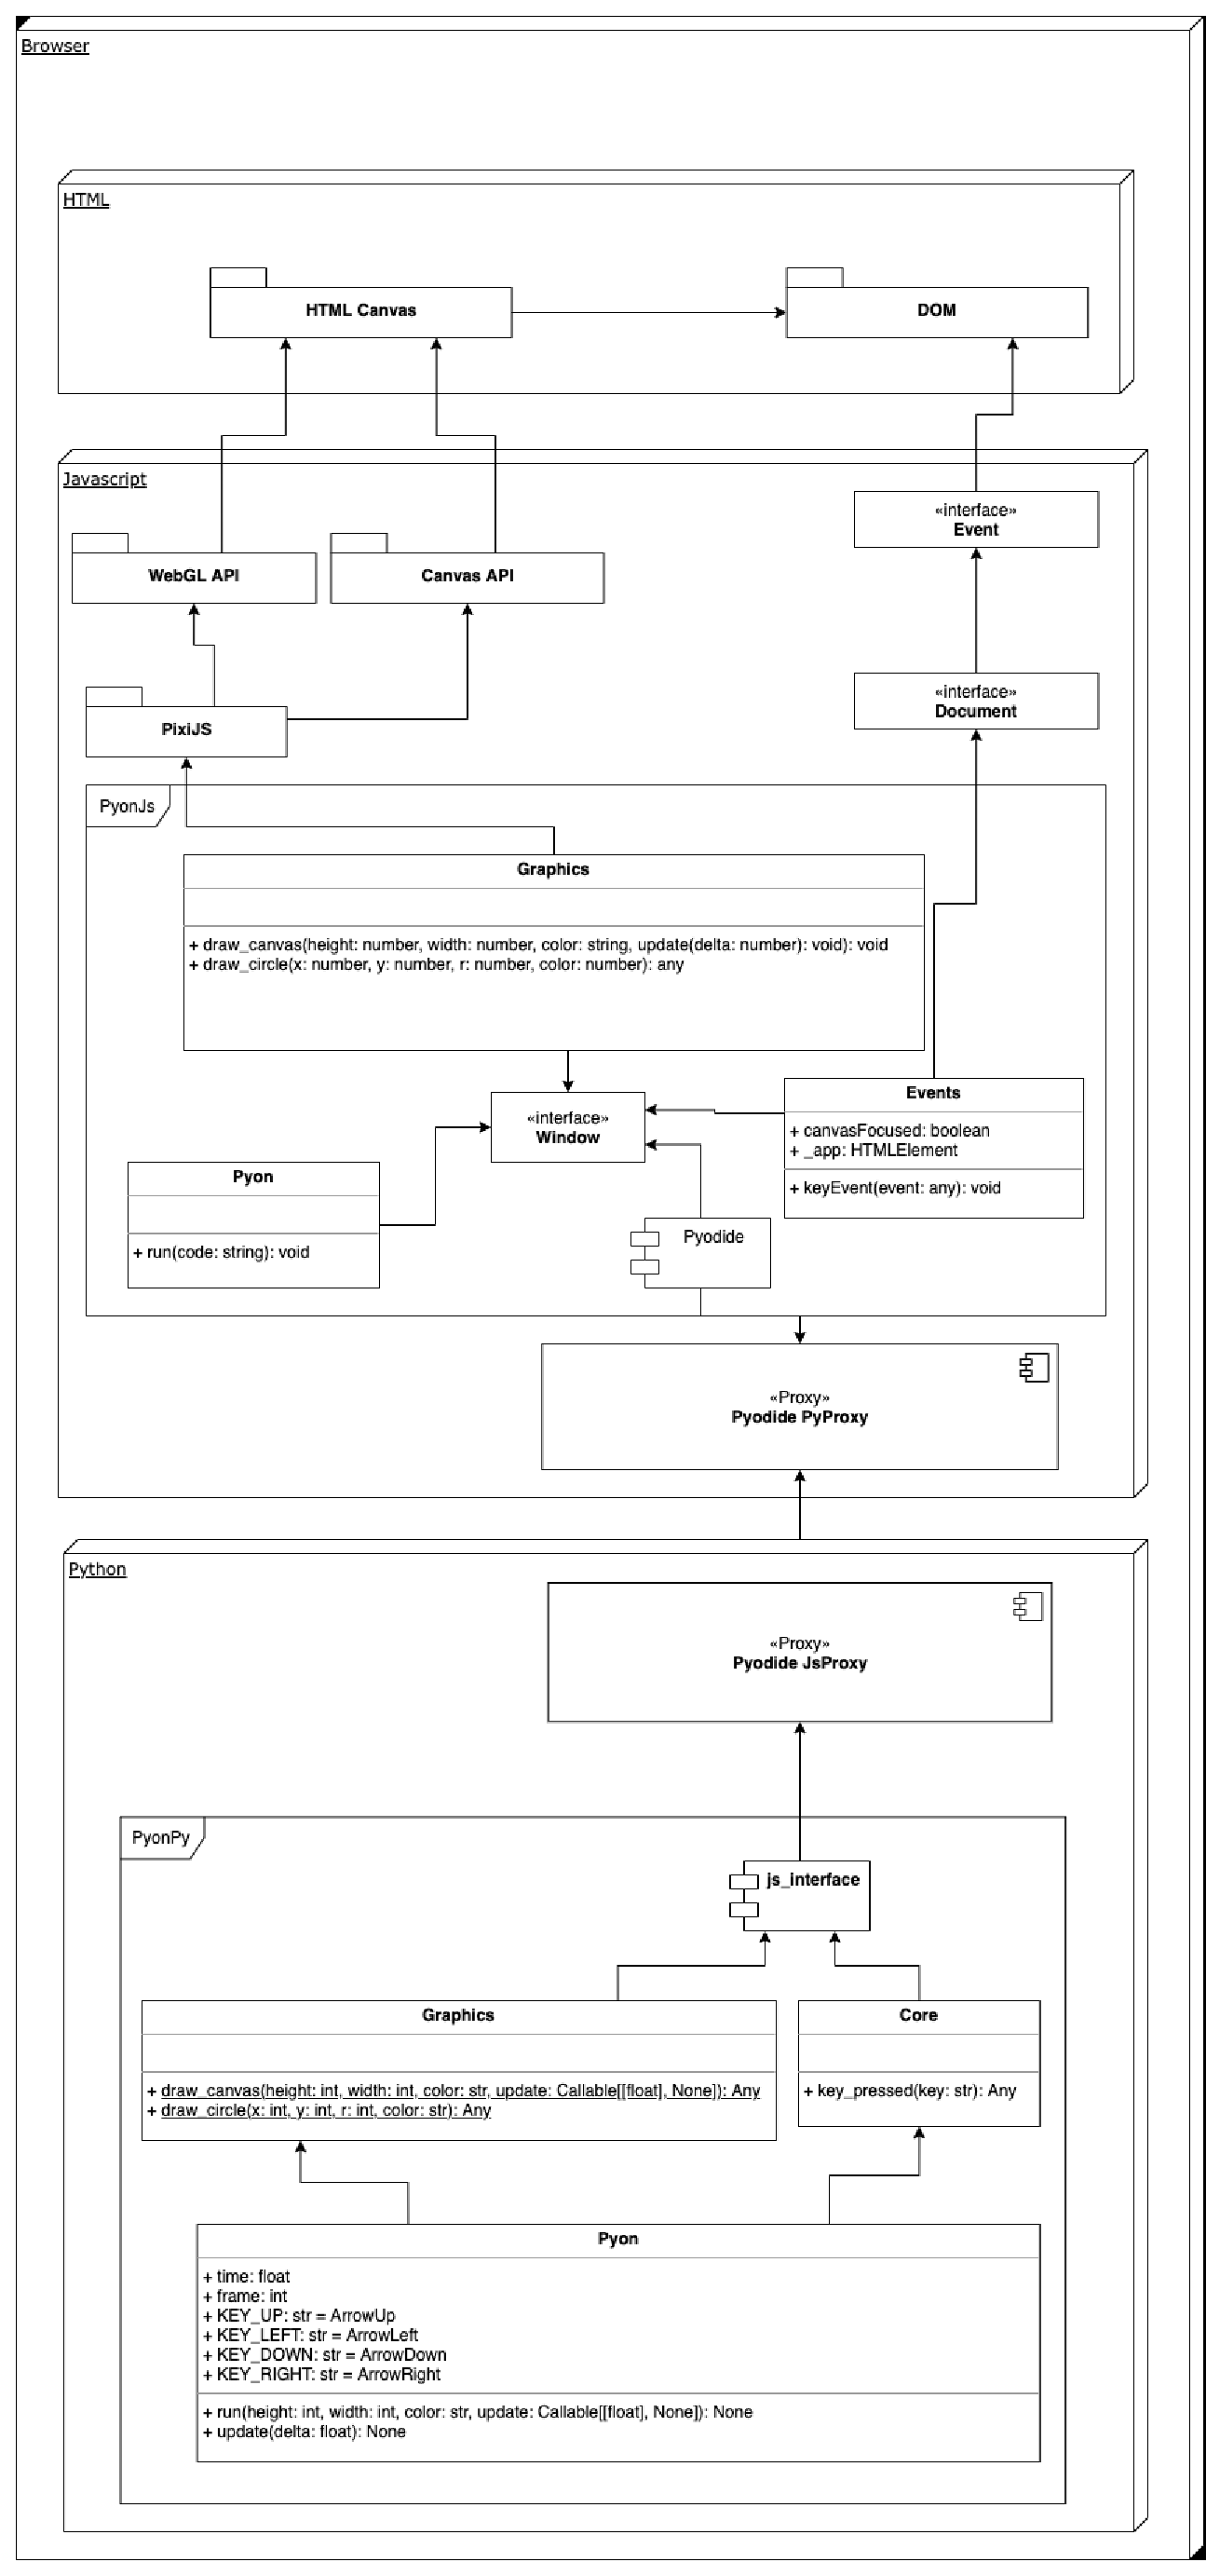
\includegraphics[trim={0 23cm 0 0},clip,keepaspectratio=true,scale=0.8]{figuras/Arquitetura.eps}
    \legend{Fonte: Autores}
    \label{fig:arquitetura_poc_p1}
\end{figure}

\begin{figure}[!h]
    \centering
    \caption{Visão Geral - Parte 2}
    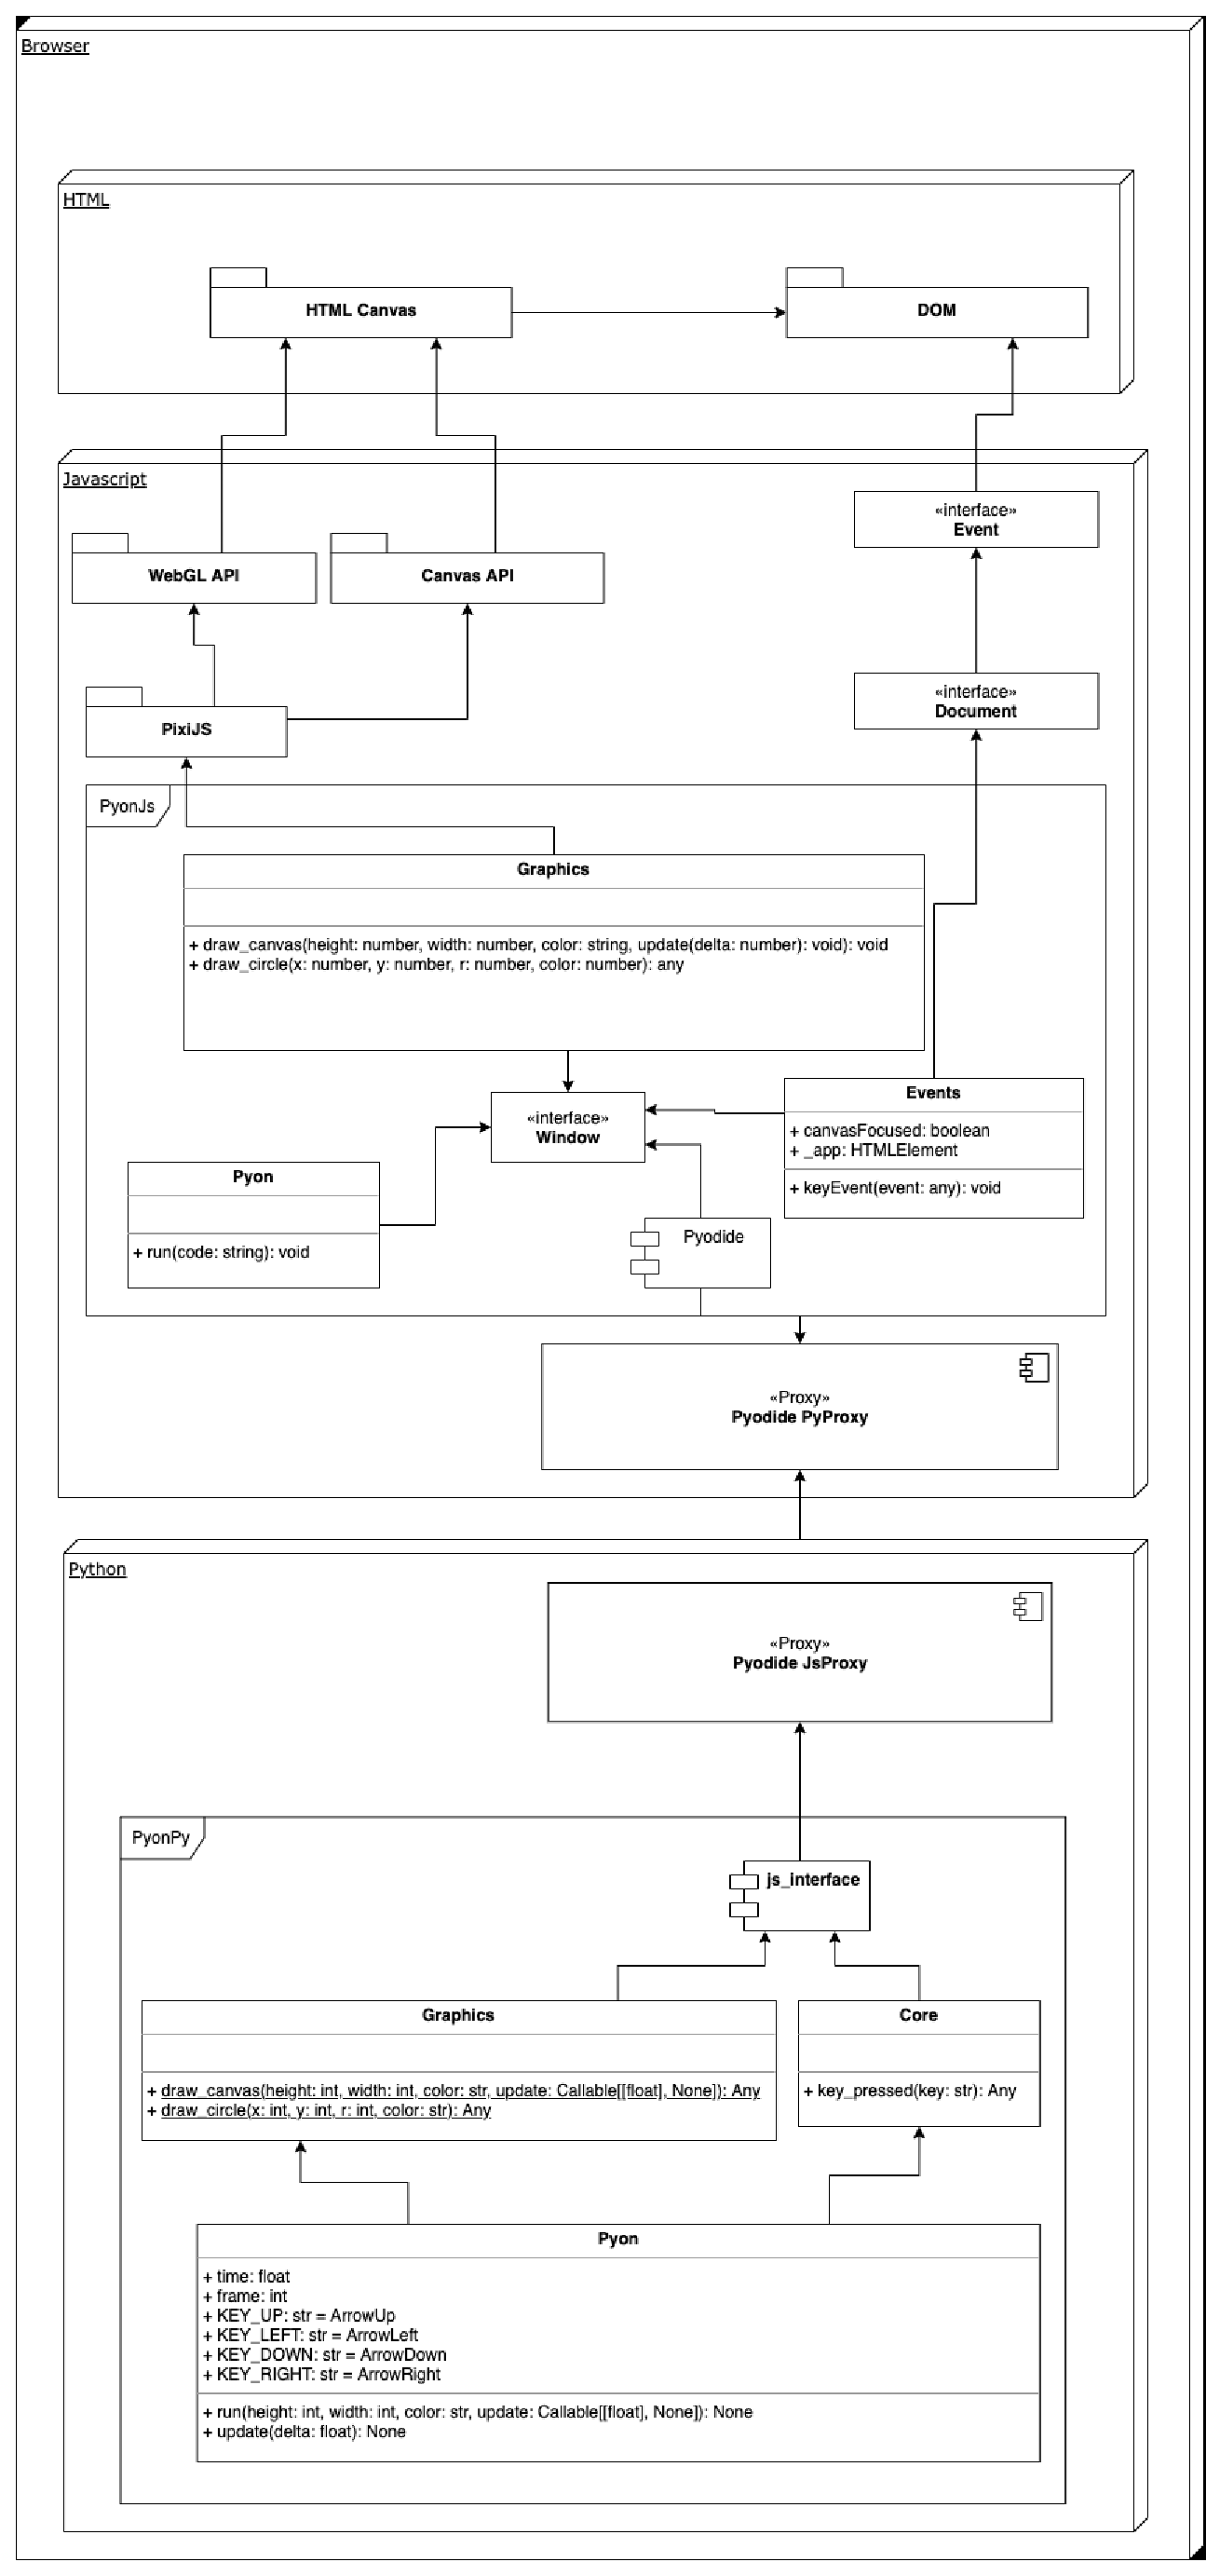
\includegraphics[trim={0 0 0 22cm},clip,keepaspectratio=true,scale=0.8]{figuras/Arquitetura.eps}
    \legend{Fonte: Autores}
    \label{fig:arquitetura_poc_p2}
\end{figure}

\section{Arquitetura}

\subsection{Camada Browser}

Representa a comunicação entre as sub-camadas HTML, JavaScript e Python. Com o python sendo interpretado para código C e compilado para Web Assembly pelo Pyodide.

\subsubsection{Camada HTML}

Representa a comunicação entre dois principais componentes HTML Canvas e DOM.

\begin{itemize}
    \item \textbf{HTML Canvas:} responsável por possibilitar a rendenização de objetos 2D na DOM.
    \item \textbf{DOM:} responsável por representar os objetos e captura de interações do usuário.
\end{itemize}

\subsection{Camada JavaScript}

Representa a comunicação da Engine na camada JavaScript. \href{https://github.com/Enpyre/engine}{EnpyreJS}

\begin{itemize}
    \item \textbf{Graphics:} Interface de comunicação entre a engine e o PixiJS, com suas funções disponibilizadas de forma global no Window.
    \item \textbf{Events:} Interface para monitoramento dos eventos de interação com a DOM, sendo o estado de cada evento atualizado de forma global no Window.
    \item \textbf{Enpyre:} Interface da engine onde seu propósito é compilar o código criado pelo aluno através da instância disponívei no Window do Pyodide.
\end{itemize}

\subsection{Camada Python}

Representa a comunicação da engine na camada Python. Todo o código do usuário vai interagir com esta camada, e não com o JavaScript. \href{https://github.com/Enpyre/engine}{EnpyrePy}

\begin{itemize}
    \item \textbf{Graphics:} Interface de comunicação entre a engine e o Graphics da camada de JavaScript.
    \item \textbf{Core:} Interface para monitoramento dos eventos de interação entre a engine e o Events da camada JavaScript.
    \item \textbf{Enpyre:} Interface que implementa atributos e funcionalidades que estarão disponíveis durante a execução do código recebido pelo Enpyre da camada JavaScript.
\end{itemize}

%
% Resultados da Prova de Conceito
%

\chapter[Resultados da Prova de Conceito]{Resultados da Prova de Conceito}
\label{apendice:resultados_poc}

O presente capítulo exibe os resultados obtidos após a concepção da Prova de Conceito.

\begin{figure}[!ht]
    \centering
    \caption{Move Ball Game}
    \includegraphics[keepaspectratio=true,scale=0.6]{figuras/code_example.eps}
    \legend{Fonte: Autores}
    \label{fig:arquitetura_poc_code}
\end{figure}

\section{Aparencia}

A Figura \ref{fig:code} exibe um navegador aberto e dois elementos principais: um canvas, acima, contendo a saída do programa; e um editor de texto, abaixo, contendo o código escrito pelo usuário. O resultado do programa permite que o usuário interaja com o círculo desenhado, usando as teclas direcionais para alterar a direção em que a bola se move.

\section{Nome da Ferramenta: Enpyre}

Inicialmente foi dado o nome Pyon, que teve a origem descrita a seguir. Primeiro, pensou-se na ferramenta como um ``motor'' (\textit{engine}, em inglês) de jogos escrito em Python. Este conceito foi alterado no princípio do trabalho, mas por sua razão adotou-se o nome provisório \textbf{Pyengine}.

Posteriormente, quando se consolidou o uso da biblioteca Pyodide, o nome provisório foi alterado para
\textbf{Pyongine}, uma mesca do nome anterior com o nome da biblioteca.

Buscando-se simplificar o nome que se usava até então, reduziu-se Pyongine para \textbf{Pyon},
acreditando-se que sua pronúncia fosse mais agradável.

Por fim, o nome foi alterado para \textbf{Enpyre}, uma mescla de ``engine'', ``Python'' e ``React'' (a biblioteca JavaScript usada para construir a interface do usuário).

\section{Estrutura Visual}

A aplicação é constituída por duas partes principais: um canvas, onde elementos podem ser desenhados, e um editor de texto integrado, com realce de sintaxe, onde o código Python pode ser escrito e executado.

\section{Resultados}

A prova de conceito comprovou a viabilidade do projeto, que mistura elementos e contextos do JavaScript e Python graças a dois proxies existentes no Pyodide.

Foi possível desenhar círculos coloridos no Canvas à partir de código Python escrito e executado à partir do editor de texto integrado. A execução segue a ordem a seguir.

\begin{enumerate}
    \item O código Python é extraído do editor de texto via JavaScript.
    \item O código Python então é interpretado pelo Pyodide, e executado em seguida.
    \item A execução do código Python inclui o download, via gerenciador de pacotes do Python (pip), do módulo Enpyre.
    \item As funções constantes neste módulo são capazes de acessar, graças ao Pyodide, a interface
    document do JavaScript.
    \item Através desta interface, as funções do PixiJS podem ser executadas. E finalmente, pode-se desenhar gráficos 2D no Canvas do DOM. As funções da parte Python do módulo Enpyre expõe estas funcionalidades de uma maneira conveniente.
\end{enumerate}

\end{apendicesenv}
